   \ \\ [-5mm]
   \begin{enumerate}
      \item Voici le tableau complété : \\ \smallskip
         {\footnotesize
         \hautab{2}
         \begin{tabular}{|*{7}{c|}}
            \hline
             & & Sport & \pscircle[fillstyle=solid,fillcolor=Gold](0,0.1){0.2} & \pscircle[fillstyle=solid,fillcolor=lightgray](0,0.1){0.2} & \pscircle[fillstyle=solid,fillcolor=brown](0,0.1){0.2} & T. \\
            \hline
            1 & 
\includegraphics[scale=0.3]{../../S06_Interpreter_representer_des_donnees/Images/S1} & {\blue Escrime} & \, {\blue 32} \, & \, 51 \, & \, 35 \, & \, {\bf 118} \, \\
            \hline
            2 & 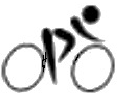
\includegraphics[scale=0.3]{../../S06_Interpreter_representer_des_donnees/Images/S2} & {\blue Cyclisme} & 41 & {\blue 27} & 23 & {\bf 91} \\
            \hline
            3 & 
\includegraphics[scale=0.3]{../../S06_Interpreter_representer_des_donnees/Images/S3} & {\blue Athlétisme} & 14 & 25 & {\blue 29} & {\bf 68} \\
            \hline
            4 & 
\includegraphics[scale=0.3]{../../S06_Interpreter_representer_des_donnees/Images/S4} & {\blue Équitation} & 14 & 13 & 10 & {\blue \bf 37} \\
            \hline
            5 & 
\includegraphics[scale=0.3]{../../S06_Interpreter_representer_des_donnees/Images/S5} & {\blue Judo} & 14 & 10 & {\blue 25} & {\bf 49} \\
            \hline
            6 & 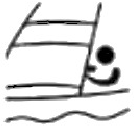
\includegraphics[scale=0.3]{../../S06_Interpreter_representer_des_donnees/Images/S6} & {\blue Voile} & 13 & {\blue 11} & 17 & {\bf 41} \\
            \hline
            7 & 
\includegraphics[scale=0.3]{../../S06_Interpreter_representer_des_donnees/Images/S7} & {\blue Tir} & {\blue 9} & 14 & 10 & {\bf 33} \\
            \hline
            8 & 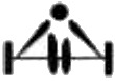
\includegraphics[scale=0.3]{../../S06_Interpreter_representer_des_donnees/Images/S8} & {\blue Haltérophilie} & 9 & {\blue 3} & 3 & {\bf 15} \\
            \hline
            9 & 
\includegraphics[scale=0.3]{../../S06_Interpreter_representer_des_donnees/Images/S9} & {\blue Natation} & 8 & 15 & {\blue 20} & {\bf 43} \\
            \hline
            10 & 
\includegraphics[scale=0.3]{../../S06_Interpreter_representer_des_donnees/Images/S10} & {\blue Canoé-kayak} & 8 & 9 & 19 & {\blue \bf 36} \\
            \hline
         \end{tabular}} \medskip
      \item Le classement des sports est établi grâce au {\blue nombre de médailles d'or}, puis d'argent, puis de bronze.
      \item On récapitule dans un tableau les angles : \\ \smallskip
   \end{enumerate}
      \small
      {\hautab{1.5}
      \begin{Ltableau}{0.95\linewidth}{5}{c}
         \hline
         Couleur & Or & Argent & Bronze & Total \\
         \hline
         Cyclisme & 41 & 27 & 23 & 91 \\
         Angle & \textcolor{blue}{\udeg{162}} & \textcolor{blue}{\udeg{107}} & \textcolor{blue}{\udeg{91}} & \udeg{360} \\
         \hline
         Tir & 9 & 14 & 10 & 33 \\
         Angle & \textcolor{blue}{\udeg{98}} & \textcolor{blue}{\udeg{153}} & \textcolor{blue}{\udeg{109}} & \udeg{360} \\
         \hline
         Canoé-kayak & 8 & 9 & 19 & 36 \\
         Angle & \textcolor{blue}{\udeg{80}} & \textcolor{blue}{\udeg{90}} & \textcolor{blue}{\udeg{190}} & \udeg{360} \\
        \hline
      \end{Ltableau}}
      {\psset{unit=0.4}
      \begin{pspicture}(-2,-3.3)(3,3.8)
         \pscircle(0,0){3}
         \pswedge[fillstyle=solid,fillcolor=Gold](0,0){3}{0}{162}
         \pswedge[fillstyle=solid,fillcolor=lightgray](0,0){3}{162}{269}
         \pswedge[fillstyle=solid,fillcolor=brown](0,0){3}{269}{360}
      \end{pspicture}
      \begin{pspicture}(-3.5,-3)(3,3.5)
         \pscircle(0,0){3}
         \pswedge[fillstyle=solid,fillcolor=Gold](0,0){3}{0}{98}
         \pswedge[fillstyle=solid,fillcolor=lightgray](0,0){3}{98}{251}
         \pswedge[fillstyle=solid,fillcolor=brown](0,0){3}{251}{360}
      \end{pspicture}
      \begin{pspicture}(-3.5,-3)(2.5,3.5)
         \pscircle(0,0){3}
         \pswedge[fillstyle=solid,fillcolor=Gold](0,0){3}{0}{80}
         \pswedge[fillstyle=solid,fillcolor=lightgray](0,0){3}{80}{170}
         \pswedge[fillstyle=solid,fillcolor=brown](0,0){3}{170}{360}
      \end{pspicture}} \\
      \quad {\blue Cyclisme \hfill Tir \hfill Canoé-kayak} \hspace*{4mm} \\ \medskip
      On remarque par exemple que chacun de ces sports à une couleur très dominante : l'or pour le cyclisme, l'argent pour le tir et le bronze pour le canoé-kayak.
